\section{Блок №1. Метод кубической аппроксимации}

\subsection{Постановка задачи}

\textbf{ДЗ1.1 (2 балла).} Выполнить решение методом кубической аппроксимации. Написать программу, генерирующую последовательность приближений, используя $\varepsilon = 0.0001$ для критерия останова.

\textbf{ДЗ1.2 (1 балл).} Реализовать визуализацию исходной и аппроксимирующей функций в одной координатной плоскости для нескольких итераций алгоритма.

Данные по варианту:
\begin{equation}\label{eq:func1}
    f(x) = \frac{1}{x} + e^x, \quad [a, b] = [0.5,\, 1.5].
\end{equation}

\subsection{Математическая модель}

Метод кубической аппроксимации основан на построении кубического полинома, интерполирующего значения функции и её производной на концах отрезка $[a, b]$.

Пусть $h = b - a$. Для концов отрезка известны $f(a)$, $f'(a)$, $f(b)$, $f'(b)$. Строится кубический полином:
\begin{equation}
    P(x) = f(a) + f'(a)(x - a) + A(x - a)^2 + B\frac{(x - a)^3}{h},
\end{equation}
где коэффициенты $A$ и $B$ определяются из условий интерполяции:
\begin{equation}
    s = \frac{f(b) - f(a)}{h}, \quad
    A = \frac{3s - f'(b) - 2f'(a)}{h}, \quad
    B = \frac{f'(b) + f'(a) - 2s}{h}.
\end{equation}

Минимум кубического полинома на $[a, b]$ находится из условия $P'(x) = 0$:
\begin{equation}
    P'(x) = f'(a) + 2A(x - a) + 3B\frac{(x - a)^2}{h} = 0.
\end{equation}

Дискриминант: $\Delta = A^2 - 3f'(a)B/h$. Корень:
\begin{equation}
    x_{new} = a + \frac{-A + \sqrt{\Delta}}{3B/h} \cdot h,
\end{equation}
с ограничением $x_{new} \in [a + 0.01h,\, b - 0.01h]$.

После вычисления $f'(x_{new})$:
\begin{itemize}
    \item Если $f'(x_{new}) < 0$, то минимум правее: $a \leftarrow x_{new}$.
    \item Если $f'(x_{new}) > 0$, то минимум левее: $b \leftarrow x_{new}$.
\end{itemize}
Критерий останова: $|f'(x_{new})| < \varepsilon$.

\subsection{Результаты}

\begin{table}[H]
    \centering
    \caption{История итераций метода кубической аппроксимации}
    \label{tab:cubic_history}
    \begin{tabular}{|c|c|c|c|c|c|}
        \hline
        \textbf{Итерация} & \textbf{$a$} & \textbf{$b$} & \textbf{$x_{new}$} & \textbf{$f(x_{new})$} & \textbf{$f'(x_{new})$} \\
        \hline
        нач. & 0.500000 & 1.500000 & --- & --- & --- \\
        1 & 0.500000 & 1.500000 & 0.751846 & 3.450971 & $3.52 \times 10^{-1}$ \\
        2 & 0.500000 & 0.751846 & 0.699252 & 3.442347 & $-3.29 \times 10^{-2}$ \\
        3 & 0.699252 & 0.751846 & 0.703480 & 3.442277 & $9.41 \times 10^{-5}$ \\
        \hline
    \end{tabular}
\end{table}

Итоговый результат:
\begin{equation}\label{eq:cubic_result}
    x^* = 0.70347954, \quad f(x^*) = 3.44227730, \quad f'(x^*) = 9.41 \times 10^{-5}.
\end{equation}

Метод сошёлся за 3 итерации. Критерий останова $|f'(x^*)| < 10^{-4}$ выполнен.

\subsection{Визуализация (ДЗ1.2)}

На рисунке~\ref{fig:cubic_all} показаны исходная функция $f(x) = 1/x + e^x$ и кубическая аппроксимация на итерациях 1 и~3. Зелёные точки обозначают границы текущего отрезка $[a, b]$, оранжевая звезда --- новое приближение $x_{new}$.

\begin{figure}[H]
    \centering
    \begin{subfigure}{0.48\textwidth}
        \centering
        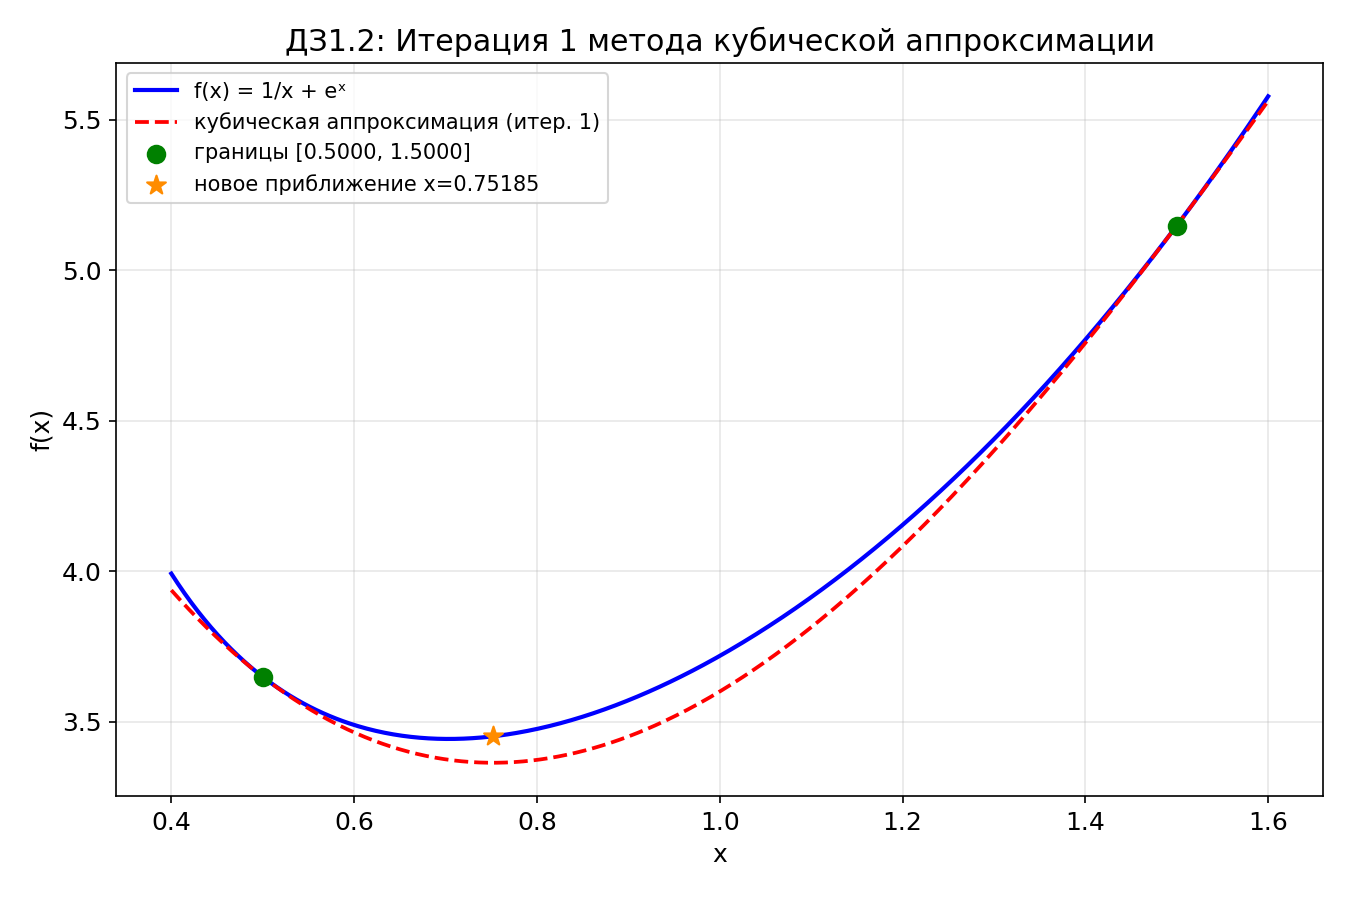
\includegraphics[width=\textwidth]{pic/iteration_1.png}
        \caption{Итерация 1: кубическая аппроксимация на $[0.5, 1.5]$}
        \label{fig:iter1}
    \end{subfigure}
    \hfill
    \begin{subfigure}{0.48\textwidth}
        \centering
        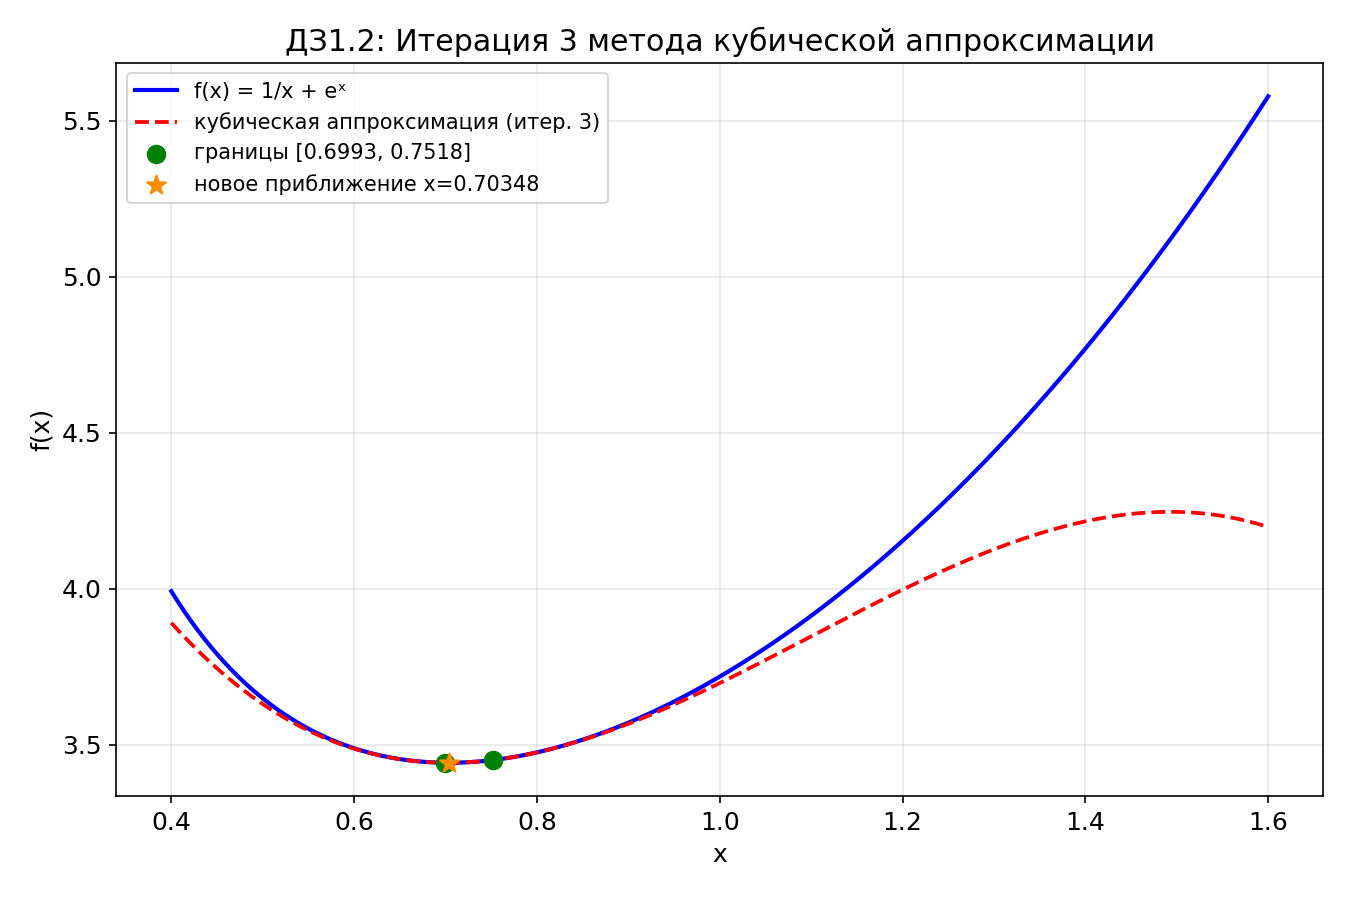
\includegraphics[width=\textwidth]{pic/iteration_3.png}
        \caption{Итерация 3: кубическая аппроксимация на $[0.6993, 0.7518]$}
        \label{fig:iter3}
    \end{subfigure}
    \caption{ДЗ1.2: Визуализация итераций метода кубической аппроксимации}
    \label{fig:cubic_all}
\end{figure}

Видно, как отрезок сужается вокруг точки минимума. На третьей итерации кубическая аппроксимация практически совпадает с исходной функцией в окрестности минимума.

\subsection{Вывод}

Метод кубической аппроксимации показал быструю сходимость: всего 3 итерации для достижения точности $\varepsilon = 10^{-4}$. Метод эффективен для гладких унимодальных функций, так как использует информацию о производных на границах отрезка, что даёт высокую точность локализации минимума на каждой итерации.
